\documentclass{article}
\usepackage[utf8]{inputenc} %кодировка
\usepackage[T2A]{fontenc}
\usepackage[english,russian]{babel} %русификатор 
\usepackage{mathtools} %библиотека матеши
\usepackage[left=1cm,right=1cm,top=2cm,bottom=2cm,bindingoffset=0cm]{geometry} %изменение отступов на листе
\usepackage{amsmath}
\usepackage{graphicx} %библиотека для графики и картинок
\graphicspath{}
\DeclareGraphicsExtensions{.pdf,.png,.jpg}
\usepackage{subcaption}
\usepackage{pgfplots}
\usepackage{float}
\usepackage{multirow}
\usepackage{listings}
\usepackage{xcolor}

\lstset{
    backgroundcolor=\color{white},   % Цвет фона
    basicstyle=\footnotesize\ttfamily, % Шрифт
    breaklines=true,                  % Перенос строк
    frame=single,                     % Рамка вокруг кода
}


\begin{document}
% НАЧАЛО ТИТУЛЬНОГО ЛИСТА
\begin{center}
    \Large
    Федеральное государственное автономное \\
    образовательное учреждение высшего образования \\ 
    «Научно-образовательная корпорация ИТМО»\\
    \vspace{0.5cm}
    \large
    Факультет программной инженерии и компьютерной техники \\
    Направление подготовки 09.03.04 Программная инженерия \\
    \vspace{1cm}
    \Large
    \textbf{Отчёт по лабораторной работе № 1} \\
    По дисциплине «Моделирование» (семестр 5)\\
    \large
    \vspace{8cm}

    \begin{minipage}{.33\textwidth}
    \end{minipage}
    \hfill
    \begin{minipage}{.4\textwidth}
    
        \textbf{Студенты}: \vspace{.1cm} \\
        \ Дениченко Александр P3312\\
        \ Балин Артём P3312\\
        \ Кобелев Роман P3312\\
        \textbf{Практик}:  \\
        \ Мартынчук Илья Геннадьевич
    \end{minipage}
    \vfill
Санкт-Петербург\\ 2024 г.
\end{center}
\pagestyle{empty}
% КОНЕЦ ТИТУЛЬНОГО ЛИСТА 
\newpage
\pagestyle{plain}

\section*{Цель работы}
Изучение методов обработки и статистического анализа результатов
измерений на примере заданной числовой последовательности путем оценки
числовых моментов и выявления свойств последовательности на основе
корреляционного анализа, а также аппроксимация закона распределения заданной
последовательности по двум числовым моментам случайной величины.

\section*{Порядок выполнения работы}
В процессе исследований необходимо выполнить обработку заданной
числовой последовательности (ЧП) для случаев, когда путем измерений получено
10, 20, 50, 100, 200 и 300 значений случайной величины, а именно:
\begin{itemize}
    \item рассчитать значения следующих числовых моментов заданной числовой
    последовательности: 
    \begin{itemize}
        \item математическое ожидание;
        \item дисперсию;
        \item среднеквадратическое отклонение;
        \item коэффициент вариации;
        \item доверительные интервалы для оценки математического ожидания с доверительными вероятностями 0,9; 0,95 и 0,99;
        \item относительные отклонения (в процентах) полученных значений от наилучших значений, полагая, что наилучшими (эталонными) являются значения, рассчитанные для наиболее представительной выборки из трехсот случайных величин;
    \end{itemize}
    \item построить график значений для заданной числовой последовательности и
    определить ее характер, а именно: является эта последовательность
    возрастающей/убывающей, периодичной (при наличии периодичности
    оценить по графику длину периода);
    \item выполнить автокорреляционный анализ и определить, можно ли
    заданную числовую последовательность считать случайной;
    \item построить гистограмму распределения частот для заданной числовой
    последовательности;
    \item  выполнить аппроксимацию закона распределения заданной случайной
    последовательности по двум начальным моментам, используя, в
    зависимости от значения коэффициента вариации, одно из следующих
    распределений:
    \begin{itemize}
        \item равномерный;
        \item экспоненциальный;
        \item нормированный Эрланга k-го порядка или гипоэкспоненциальный с
        заданным коэффициентом вариации;
        \item гиперэкспоненциальный с заданным коэффициентом вариации;
    \end{itemize}
    \item реализовать генератор случайных величин в соответствии с полученным
    аппроксимирующим законом распределения (в EXEL или программно) и
    проиллюстрировать на защите его работу;
    \item сгенерировать последовательность случайных величин в соответствии с
    полученным законом распределения и рассчитать значения числовых
    моментов по аналогии с заданной числовой последовательностью;
    \item выполнить
    автокорреляционный
    анализ
    сгенерированной
   последовательности случайных величин;
    \item выполнить сравнительный анализ сгенерированной последовательности
    случайных величин с заданной последовательностью, построив
    соответствующие зависимости на графике значений и гистограмме
    распределения частот; 
    \item  оценить корреляционную зависимость сгенерированной и заданной
    последовательностей случайных величин.
\end{itemize}
Результаты проводимых исследований представить в виде таблиц и графиков.
\\ \\

На основе полученных промежуточных и конечных результатов следует
сделать обоснованные выводы об исследуемой числовой последовательности,
предложить закон распределения для ее описания и оценить качество
аппроксимации этим законом.

\section{Оценки и доверительные интервалы}
\begin{table}[H]
    \centering
    \caption{Расчетные характеристики}
    \begin{tabular}{|l|l|}
    \hline
    Характеристика & Формула \\
    \hline
    Оценка мат ожидания & $\widetilde{m}  = \frac{1}{n} \sum_{i=1}^{n} X_i$ \\
    \hline
    Оценка дисперсии & $\widetilde{D} = \frac{1}{n-1} \sum_{i=1}^{n} (X_i - \widetilde{m})^2$ \\
    \hline
    Среднеквадратическое отклонение & $\sigma = \sqrt{D}$ \\
    \hline
    Коэффициент вариации & $V = \frac{\sigma}{m} \times 100\%$ \\
    \hline
    Оценка среднеквадратического отклонения мат ожидания & $\widetilde{\sigma_m} = \sqrt{\frac{\widetilde{D}}{n}}$ \\
    \hline
    Отклонение & $\epsilon_p = t_p \cdot \widetilde{\sigma_m}$, $t_p$ = Ф'($\frac{1 + p}{2}$)  \\
    \hline
    Доверительный интервал & $m \pm \epsilon_p$ \\
    \hline
    Доверительный интервал (0.9) & $m \pm 1.643\cdot \widetilde{\sigma_m}$ \\
    \hline
    Доверительный интервал (0.95) & $m \pm 1.960\cdot \widetilde{\sigma_m}$ \\
    \hline
    Доверительный интервал (0.99) & $m \pm 2.576\cdot \widetilde{\sigma_m}$ \\
    \hline
    \end{tabular}
    \end{table}


\begin{table}[H]
    \centering
    \caption{Форма 1. Характеристики заданной ЧП (вариант 2)}
    \begin{tabular}{|l|c|c|c|c|c|c|c|}
    \hline
    \multirow{2}{*}{Характеристика}& & \multicolumn{6}{c|}{Количество случайных величин} \\
    \cline{3-8}
    & & 10 & 20 & 50 & 100 & 200 & 300 \\
    \hline
    Мат. ож. & Знач. & 147.844 & 181.747 & 146.786 & 165.879 & 173.955 & 168.836 \\
     & \%            & -12.433 & 7.647 & -13.06 & -1.751 & 3.032 &  \\ 
    \hline
    Дов. инт. (0,9) & Знач.& $\pm$30.879 & $\pm$46.27 & $\pm$21.414 & $\pm$16.096 & $\pm$13.063 & $\pm$11.039 \\
     & \%                  & 179.712 & 319.132 & 93.982 & 45.807 & 18.332 &  \\
    \hline
    Дов. инт. (0,95) & Знач.& $\pm$36.836 & $\pm$55.197 & $\pm$25.546 & $\pm$19.202 & $\pm$15.584 & $\pm$13.169 \\
     & \%                   & 179.712 & 319.132 & 93.982 & 45.807 & 18.332 &  \\
    \hline
    Дов. инт. (0,99) & Знач.& $\pm$48.413 & $\pm$72.545 & $\pm$33.575 & $\pm$25.237 & $\pm$20.481 & $\pm$17.308 \\
     & \%                   & 179.712 & 319.132 & 93.982 & 45.807 & 18.332 &  \\
    \hline
    Дисперсия & Знач. & 3532.136 & 15861.648 & 8493.935 & 9597.771 & 12643.022 & 13543.708\\
     & \%             & -73.92 & 17.115 & -37.285 & -29.135 & -6.65 &  \\
    \hline
    С.к.о. & Знач. & 59.432 & 125.943 & 92.163 & 97.968 & 112.441 & 116.377\\
     & \%          & -48.932 & 8.219 & -20.807 & -15.819 & -3.382 &  \\
    \hline
    К-т вариации & Знач. & 0.402 & 0.693 & 0.628 & 0.591 & 0.646 & 0.689\\
     & \%                & -41.681 & 0.532 & -8.911 & -14.318 & -6.226 &  \\
    \hline
    \multicolumn{7}{l}{\footnotesize \% - относительное отклонение рассчитанных значений от значений,}\\
    \multicolumn{7}{l}{\footnotesize полученных для выборки из трехсот величин}
    \end{tabular}
    \end{table}

    Чем больше значений берется в выборке, тем точнее рассчитываются параметры.
    Значение коэффициента вариации приближено к 1, но все же меньше
    единицы.

\section{График значений заданной ЧП}

\begin{figure}[ht]
    \centering
    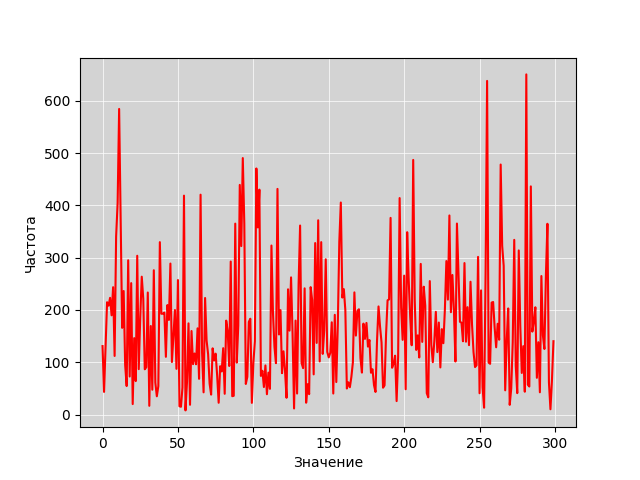
\includegraphics[width=.8\textwidth]{1}
    \caption{График значений заданной ЧП}
\end{figure}

График отображает значения числовой последовательности из 300 элементов.
\\ \\
\textbf{Промежуточный вывод:}
\begin{itemize}
    \item Значения колеблются вокруг некоторого среднего значения, не проявляя устойчивого роста или падения на протяжении всей последовательности.
    \item Хотя на графике наблюдаются некоторые повторяющиеся участки, нельзя сказать, что последовательность имеет четко выраженный период. Колебания выглядят довольно случайными.
    \item На графике видны несколько пиков, где значения значительно превышают средний уровень. Это говорит о наличии выбросов в данных.
    \item Амплитуда колебаний достаточно велика, что свидетельствует о значительной изменчивости данных.
\end{itemize}
Стационарна (среднее значение и дисперсия постоянны во времени), но не периодическая.


\section{Результаты автокорреляционного анализа}

Расчёты коэффицентов автокорреляции происходили по следующей формуле:
\[r_{xk} \approx \frac{\sum_{i=1}^{n}(x_i - M[X])(x_{i+k} - M[X])}{\sum_{i=1}^{n}(x_i - M[X])^2}\]

\begin{table}[H]
    \centering
    \caption{Форма 3. Коэффициенты автокорреляции}
    \begin{tabular}{|c|c|c|c|c|c|c|c|c|c|c|}
        \hline
        Сдвиг ЧП & 1 & 2 & 3 & 4 & 5 & 6 & 7 & 8 & 9 & 10\\
        \hline
        К-т АК для задан. ЧП & 0.0916 & 0.0318 & 0.0306 & -0.0143 & -0.0345 & -0.0452 & -0.0496 & 0.0065 & 0.0905 & -0.0010\\
        \hline
        К-т АК для сгенерир. ЧП & 0.0892 & 0.0879 & -0.0259 & 0.0111 & -0.0955 & -0.0190 & -0.0461 & -0.0726 & -0.0091 & -0.1153\\
        \hline 
        \% & -2.62 & 176.4 & -184.6 & 177.62 & -176.81 & 57.96 & 7.06 & -1216.92 & -110.06 & -11430\\
        \hline
    \end{tabular}
\end{table}


\begin{minipage}{.48\textwidth}
    \centering
    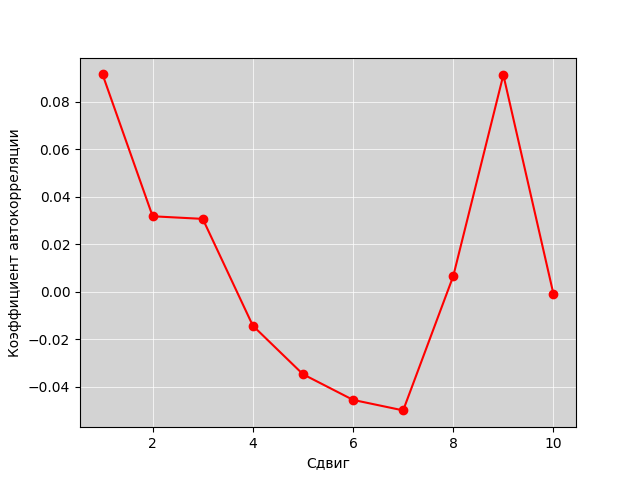
\includegraphics[width=.9\textwidth]{4}
    \captionof{figure}{\small График автокорреляции для лагов \\ 1-10 для заданной числовой последовательности}
\end{minipage}
\hfill
\begin{minipage}{.48\textwidth}
    \centering
    
\includegraphics[width=.9\textwidth]{5}
    \captionof{figure}{\small График автокорреляции для лагов 1-10 для сгенерированной числовой последовательности}
\end{minipage}
\\ \\
\\ \\
\textbf{Промежуточный вывод:}
Коэффициент автокорреляции Сдвигов ЧП от 1 до 10 приближены к нулю,
следовательно, можно сказать, что обе выборки случайны.

\section{Гистограмма распределения частот для заданной ЧП}

\begin{figure}[ht]
    \centering
    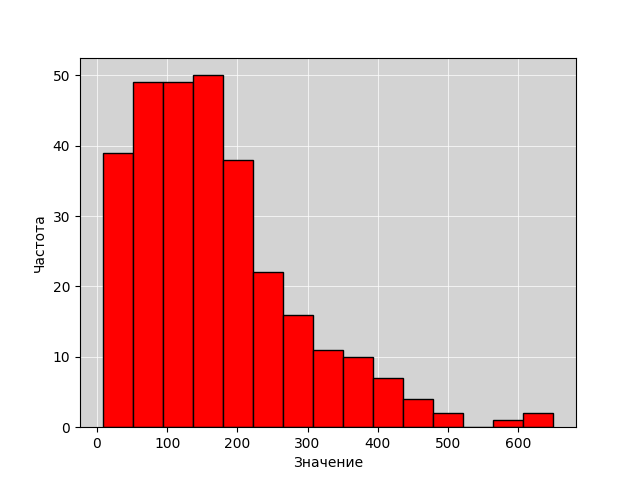
\includegraphics[width=.7\textwidth]{2}
    \caption{Гистограмма заданной ЧП}
\end{figure}


\section{Аппроксимирующий закон распределения}

Подсчитанный коэффицент вариации 0.689 < 1, при этом 0.689 > 0.577 => пробуем распределение Эрланга.
\\\\
Просчитаем параметр формы:
\[k = \left(\frac{\widetilde{m}}{\sigma}\right)^2 = \left(\frac{168.836}{116.377}\right)^2 \approx 2 \]
\\
Просчитаем параметр скорости:
\[\lambda = \left(\frac{k}{\widetilde{m}}\right) = \left(\frac{2}{168.836}\right) = 0.0118 \]
\begin{figure}[ht]
    \centering
    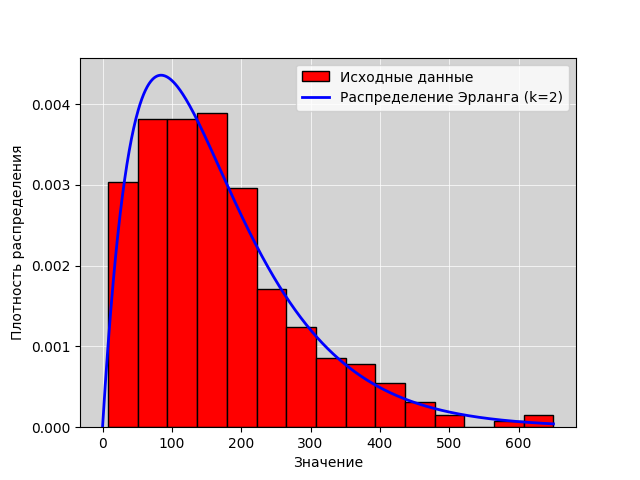
\includegraphics[width=.7\textwidth]{6}
    \caption{Гистограмма значений заданной ЧП с аппроксимацией}
\end{figure}

В результате анализа коэффициента вариации, для аппроксимации выбран закон распределения Эрланга.

\section{Описание программы для формирования новой ЧП}

\begin{lstlisting}[language=Python]
    shape_param = 2
    scale_param = d_best / m_best
    erlang_300 = np.random.gamma(shape=shape_param, scale=scale_param, size=300).tolist()
\end{lstlisting}

\section{Оценки и доверительные интервалы для новой сгенерированной ЧП}

\begin{table}[H]
    \centering
    \caption{Форма 2. Характеристики сгенерированной ЧП}
    \begin{tabular}{|l|c|c|c|c|c|c|c|}
    \hline
    \multirow{2}{*}{Характеристика}& & \multicolumn{6}{c|}{Количество случайных величин} \\
    \cline{3-8}
    & & 10 & 20 & 50 & 100 & 200 & 300 \\
    \hline
    Мат. ож. & Знач. & 83.078& 207.15& 167.297& 167.826& 160.307& 156.587 \\
     & \%            & -43.807& 13.977& 13.974& 1.174& 7.846 &\\ 
    \hline
    Дов. инт. (0,9) & Знач.& $\pm$31.385 & $\pm$63.236 & $\pm$22.575 & $\pm$22.332 & $\pm$15.128 & $\pm$10.127 \\
     & \%                  & 1.638& 36.668& 5.423& 38.743& 15.806& \\
    \hline
    Дов. инт. (0,95) & Знач.& $\pm$37.44 & $\pm$75.437 & $\pm$26.931 & $\pm$26.641 & $\pm$18.047 & $\pm$12.081 \\
     & \%                   & 1.64& 36.669& 5.422& 38.74& 15.802 & \\
    \hline
    Дов. инт. (0,99) & Знач.& $\pm$49.207 & $\pm$99.146 & $\pm$35.395 & $\pm$35.014 & $\pm$23.718 & $\pm$15.877 \\
     & \%                   & 1.64& 36.669& 5.421& 38.74& 15.806&\\
    \hline
    Дисперсия & Знач. & 3648.885 & 29627.185 & 9439.845 & 18474.982 & 16955.314 & 11396.837\\
     & \%             & -3.305& 86.785& -11.136& 92.492& 34.108  &\\
    \hline
    С.к.о. & Знач. & 60.406 & 172.125 & 97.159 & 97.968 & 135.923 & 106.756\\
     & \%          & -1.639& 36.669& -5.421& -38.742& 15.805 &\\
    \hline
    К-т вариации & Знач. & 0.727 & 0.831 & 0.581 & 0.81 & 0.812 & 0.682\\
     & \%                & 80.871& 19.902& -7.523& 37.039& 25.739 &\\
    \hline
    \multicolumn{7}{l}{\footnotesize \% - относительное отклонение рассчитанных значений от значений,}\\
    \multicolumn{7}{l}{\footnotesize полученных для выборки из трехсот величин}
    \end{tabular}
    \end{table}

Математическое ожидание отличается от математического ожидания исходной
    выборки на минимальную величину. Это говорит
    о том, что аппроксимация выполнена качественно.

\section{Результаты автокорреляционного анализа сгенерированной ЧП}

Подсчитанный коэффицент вариации 0.682 < 1, при этом 0.682 > 0.577 => пробуем распределение Эрланга.
\\\\
Просчитаем параметр формы:
\[k = \left(\frac{\widetilde{m}}{\sigma}\right)^2 = \left(\frac{156.587}{106.756}\right)^2 \approx 2 \]
\\
Просчитаем параметр скорости:
\[\lambda = \left(\frac{k}{\widetilde{m}}\right) = \left(\frac{2}{156.587}\right) = 0.0128 \]
В результате анализа коэффициента вариации, для аппроксимации выбран закон распределения Эрланга.

\section{Сравнение гистограмм}
\begin{figure}[H]
    \centering
    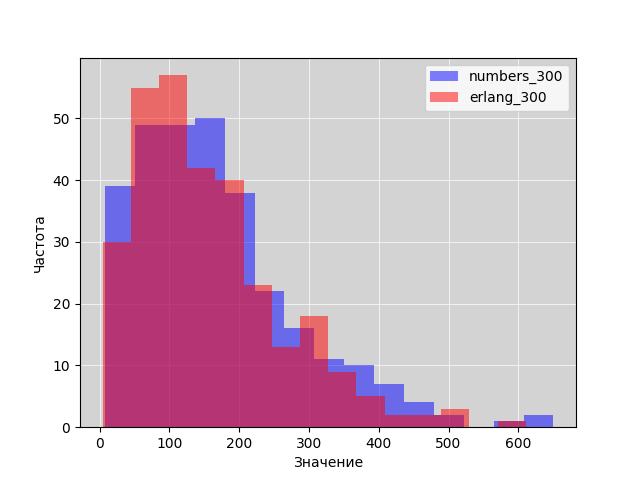
\includegraphics[width=.6\textwidth]{3}
    \caption{Гистограммы исходной и сгенерированной ЧП}
\end{figure}
Сравнивая полученные гистограммы частот, можно сделать вывод, что
сгенерированная нами последовательность практически идентична исходной (по
варианту). Тем самым можно утверждать, что выбранная нами аппроксимация
подходит.

\section*{Вывод}
Проведенный анализ показал, что исходную числовую последовательность можно считать случайной. 
Закон распределения Эрланга с параметрами k=2 и $\lambda$ = 0.0118 обеспечивает достаточно хорошую аппроксимацию исходных данных, 
что подтверждается сравнением числовых характеристик и гистограмм исходной и сгенерированной последовательностей. 
Небольшие расхождения в значениях характеристик могут быть связаны с естественной случайностью выборок и конечным размером исходной ЧП.


\end{document}
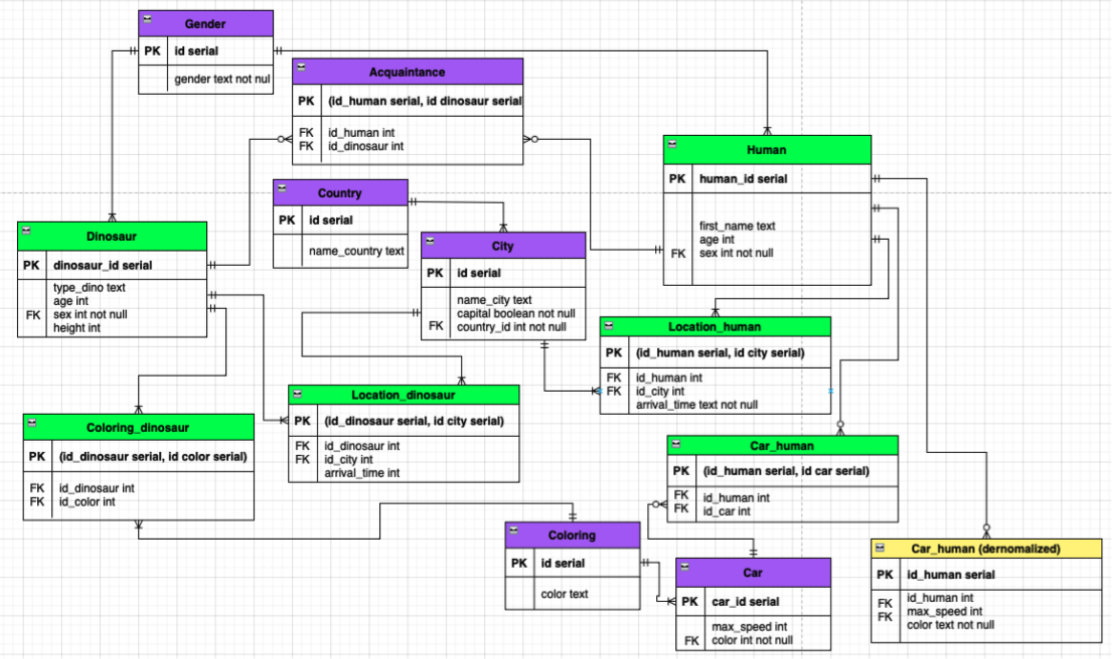
\includegraphics[width=.9\textwidth]{123}



